\documentclass[aspectratio=169]{beamer}

\usetheme{Madrid}
\usecolortheme{default}
\setbeamertemplate{navigation symbols}{}
\usepackage{eso-pic}
\usepackage[brazil]{babel}
\shorthandoff{"}
\usepackage[T1]{fontenc}
\usepackage[utf8]{inputenc}
\usepackage{lmodern}

\usepackage{tikz}
\usetikzlibrary{arrows.meta, positioning, shapes.geometric, fit, calc, backgrounds}
\usepackage{listings}
\usepackage{xcolor}

\definecolor{meuazul}{RGB}{0, 79, 151}
\definecolor{meucinza}{RGB}{80, 80, 80}
\definecolor{meuvermelhoescuro}{RGB}{180, 30, 30}
\definecolor{meuverde}{RGB}{30, 130, 60}
\setbeamercolor{structure}{fg=meuazul}

\title[Engenharia de Segurança]{Engenharia de Segurança}
\subtitle{Engenharia de Qualidade e Confiabilidade}
\author{Prof. Me. Sergio Souza Novak — UniRV}
\titlegraphic{
\includegraphics[width=2cm]{logo.png}}

\begin{document}

% Slide de Título
\frame[plain]{\titlepage}

\AddToShipoutPictureFG{
    \put(\LenToUnit{.92\paperwidth},\LenToUnit{.185\paperheight})
    {\vtop{{\null}\makebox{
\includegraphics[width=.8cm,keepaspectratio]{logo.png}}}}}

% -------------

% ===== SLIDE 1: CASO REAL =====
\begin{frame}{1) Caso Real: Aeroporto de Varsóvia}
  \begin{columns}
    \begin{column}{0.62\textwidth}
      Em \textbf{1993}, um Airbus colidiu durante o pouso no aeroporto de Varsóvia:
      \begin{itemize}
        \item \textbf{2 mortes} e \textbf{54 feridos}.
        \item Causa significativa: \alert{falha no software de controle}.
        \item O software \textbf{reduziu a eficiência do sistema de frenagem}.
        \item As condições da pista não foram corretamente interpretadas.
      \end{itemize}
      \vspace{0.3em}
      \textit{``Ilustra que o software é um componente fundamental em sistemas críticos para preservar a vida humana.''}
    \end{column}
    \begin{column}{0.35\textwidth}
      \centering
      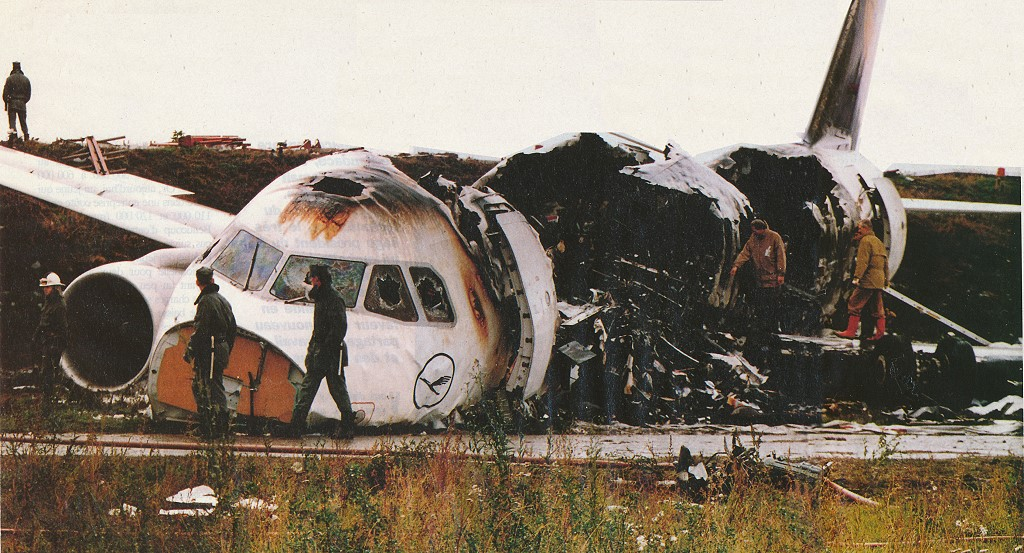
\includegraphics[width=\textwidth]{varsovia.png}

    \end{column}
  \end{columns}
\end{frame}

% ===== SLIDE 2: O QUE É SEGURANÇA (SAFETY)? =====
\begin{frame}{2) O que é Segurança (\textit{Safety})?}
  \begin{block}{Definição}
    Um sistema é considerado \textbf{seguro} se operar sem \textbf{falhas catastróficas} — falhas que causem ou possam causar morte ou lesão às pessoas.
  \end{block}
  \vspace{0.4em}
  \begin{itemize}
    \item Sistemas cujas falhas causem \textbf{danos ambientais} também são críticos em segurança.
    \item Danos ambientais (ex.: vazamento químico) podem levar a subsequentes mortes ou lesões.
    \item Segurança (\textit{safety}) é uma das principais propriedades da \textbf{dependabilidade}.
  \end{itemize}
  \vspace{0.4em}
  \begin{alertblock}{Atenção}
    \textit{Safety} $\neq$ \textit{Security}. \textbf{Safety} trata de falhas que causam danos físicos; \textbf{Security} trata de proteção contra ataques e acesso não autorizado.
  \end{alertblock}
\end{frame}

% ===== SLIDE 3: SAFETY VS DEPENDABILITY =====
\begin{frame}{3) Segurança e Dependabilidade}
  \centering
  \begin{tikzpicture}[node distance=1.4cm, every node/.style={font=\small}]
    \tikzstyle{prop} = [rectangle, rounded corners, minimum width=3.0cm, minimum height=0.9cm,
                        align=center, draw=meuazul, fill=blue!12, text=meuazul, font=\small\bfseries]
    \tikzstyle{center} = [ellipse, minimum width=3.8cm, minimum height=1.2cm,
                          align=center, draw=meuazul!80, fill=meuazul, text=white, font=\bfseries]
    \tikzstyle{arrow} = [thick, ->, >=Stealth, meuazul]

    \node (dep) [center] {Dependabilidade};
    \node (disp) [prop, above left=1.0cm and 1.6cm of dep]  {Disponibilidade};
    \node (conf) [prop, above=1.2cm of dep]        {Confiabilidade};
    \node (safe) [prop, above right=1.0cm and 1.6cm of dep] {\textcolor{meuvermelhoescuro}{Segurança (Safety)}};
    \node (manut)[prop, below left=1.0cm and 1.6cm of dep]  {Manutenibilidade};
    \node (int)  [prop, below=1.2cm of dep]        {Integridade};
    \node (seg)  [prop, below right=1.0cm and 1.6cm of dep] {Segurança (Security)};

    \draw[arrow] (dep) -- (disp);
    \draw[arrow] (dep) -- (conf);
    \draw[arrow] (dep) -- (safe);
    \draw[arrow] (dep) -- (manut);
    \draw[arrow] (dep) -- (int);
    \draw[arrow] (dep) -- (seg);
  \end{tikzpicture}
\end{frame}

% ===== SLIDE 4: DUPLO PAPEL DO SOFTWARE =====
\begin{frame}{4) O Duplo Papel do Software na Segurança}
  O software em sistemas críticos em segurança exerce \textbf{dois papéis}:

  \vspace{0.5em}
  \begin{columns}
    \begin{column}{0.48\textwidth}
      \begin{block}{Papel 1: Controle Direto}
        \begin{itemize}
          \item O sistema é \textbf{controlado por software}.
          \item Decisões do software $\Rightarrow$ ações críticas.
          \item O comportamento do software está \textbf{diretamente ligado} à segurança global.
        \end{itemize}
      \end{block}
    \end{column}
    \begin{column}{0.48\textwidth}
      \begin{block}{Papel 2: Monitoramento}
        \begin{itemize}
          \item Software \textbf{confere e monitora} outros componentes.
          \item Ex.: monitorar todos os componentes do motor de uma aeronave.
          \item Falha do software de monitoramento $\Rightarrow$ outros componentes podem falhar.
        \end{itemize}
      \end{block}
    \end{column}
  \end{columns}
\end{frame}

% ===== SLIDE 5: DIAGRAMA DUPLO PAPEL =====
\begin{frame}{5) Fluxo: Controle e Monitoramento}
  \centering
  \begin{tikzpicture}[node distance=1.2cm, every node/.style={font=\small}]
    \tikzstyle{box} = [rectangle, rounded corners, minimum width=3.2cm, minimum height=0.85cm,
                       align=center, draw=meuazul, fill=blue!10]
    \tikzstyle{boxr} = [rectangle, rounded corners, minimum width=3.2cm, minimum height=0.85cm,
                        align=center, draw=meuvermelhoescuro, fill=red!10]
    \tikzstyle{boxg} = [rectangle, rounded corners, minimum width=3.2cm, minimum height=0.85cm,
                        align=center, draw=meuverde, fill=green!10]
    \tikzstyle{arr} = [thick,->,>=Stealth]

    \node (sw)  [box]  {Software de Controle};
    \node (sys) [boxr, right=2.5cm of sw] {Sistema Físico\\(atuadores, freios…)};
    \node (mon) [boxg, below=1.5cm of sw] {Software de Monitoramento};
    \node (comp)[boxr, right=2.5cm of mon]{Componentes\\(motores, sensores…)};
    \node (safe)[box,  below=1.5cm of mon, xshift=2cm, minimum width=5cm]{Segurança Global do Sistema};

    \draw[arr, meuazul] (sw) -- node[above, font=\tiny]{comanda} (sys);
    \draw[arr, meuvermelhoescuro] (sys) -- ++(0,-0.6) -| (safe);
    \draw[arr, meuverde] (mon) -- node[above, font=\tiny]{inspeciona} (comp);
    \draw[arr, meuvermelhoescuro] (comp) -- ++(0,-0.6) -| (safe);
    \draw[arr, meucinza] (sw)  -- node[right, font=\tiny]{alimenta} (mon);
  \end{tikzpicture}
\end{frame}

% ===== SLIDE 6: CONFIABILIDADE ≠ SEGURANÇA =====
\begin{frame}{6) Confiabilidade $\neq$ Segurança}
  \begin{alertblock}{Armadilha Comum}
    Um sistema \textbf{confiável} pode \textbf{não ser seguro}, e vice-versa!
  \end{alertblock}

  \vspace{0.5em}
  \centering
  \begin{tikzpicture}[every node/.style={font=\small}]
    \tikzstyle{circulo} = [circle, minimum size=3.0cm, draw, thick, opacity=0.8]
    \begin{scope}
      \draw[fill=blue!25, draw=meuazul, thick] (-1.5, 0) circle (2.2cm);
      \draw[fill=red!25, draw=meuvermelhoescuro, thick] (1.5, 0) circle (2.2cm);
      \node[font=\small\bfseries, text=meuazul]          at (-2.6, 0) {Confiável};
      \node[font=\small\bfseries, text=meuvermelhoescuro] at ( 2.6, 0) {Seguro};
      \node[font=\tiny, align=center]                    at (0, 0) {Ideal:\\Confiável\\e Seguro};
      \node[font=\tiny, align=center, text=meuazul]      at (-2.2, 0.5) {Confiável\\mas não\\seguro};
      \node[font=\tiny, align=center, text=meuvermelhoescuro] at (2.2, 0.5) {Seguro\\mas não\\confiável};
    \end{scope}
  \end{tikzpicture}
  \vspace{0.3em}\\
  \small{O acidente em Varsóvia: o sistema era tecnicamente confiável, porém falhou em segurança.}
\end{frame}

% ===== SLIDE 7: 4 RAZÕES — SISTEMAS CONFIÁVEIS PODEM NÃO SER SEGUROS =====
\begin{frame}{7) Por que Sistemas Confiáveis Podem Não Ser Seguros?}
  Quatro razões principais:
  \begin{enumerate}
    \item \textbf{Defeitos não detectados} podem ficar inativos por anos e causar falhas inesperadas.
    \item \textbf{Especificações incompletas} não descrevem o comportamento exigido em situações críticas.
    \item \textbf{Mau funcionamento de hardware} gera sinais fora dos intervalos tratáveis pelo software.
    \item \textbf{Entradas inesperadas dos operadores} individualmente corretas, mas perigosas em combinação.
  \end{enumerate}
\end{frame}

% ===== SLIDE 8: CAUSA 1 — DEFEITOS INATIVOS =====
\begin{frame}{8) Razão 1: Defeitos Inativos (\textit{Dormant Bugs})}
  \begin{columns}
    \begin{column}{0.55\textwidth}
      \begin{itemize}
        \item Nunca podemos ter \textbf{100\% de certeza} de que um software é livre de defeitos.
        \item Defeitos podem \textbf{ficar inativos por longo tempo}.
        \item Falhas de software ocorrem \textbf{após anos} de operação confiável.
        \item Ambientes de produção revelam combinações de estados impossíveis de testar exaustivamente.
      \end{itemize}
    \end{column}
    \begin{column}{0.42\textwidth}
      \centering
      \begin{tikzpicture}[every node/.style={font=\scriptsize}]
        \draw[->, thick, meuazul] (0,0) -- (5,0) node[right]{Tempo};
        \draw[->, thick, meuazul] (0,0) -- (0,3) node[above]{Confiabilidade};
        \draw[thick, meuverde, dashed] (0,2.4) -- (3.5,2.4);
        \draw[thick, meuverde] (0,0.3) .. controls (0.8,2.6) and (1.5,2.4) .. (3.5,2.4);
        \draw[thick, meuvermelhoescuro] (3.5,2.4) .. controls (4.0,2.4) and (4.2,1.2) .. (4.6,0.3);
        \filldraw[meuvermelhoescuro] (3.5,2.4) circle (2pt);
        \node[meuvermelhoescuro, align=center] at (4.3, 1.8) {Falha\\latente};
        \node[meuverde] at (1.5, 1.2) {Estável};
      \end{tikzpicture}
    \end{column}
  \end{columns}
\end{frame}

% ===== SLIDE 9: CAUSA 2 — ESPECIFICAÇÃO INCOMPLETA =====
\begin{frame}{9) Razão 2: Especificações Incompletas}
  \begin{block}{Estudo de Lutz (1993) — Sistemas Embarcados}
    \textit{``As dificuldades com os requisitos são a causa principal dos erros de software relacionados à segurança, que persistiram até a integração e teste do sistema.''}
  \end{block}
  \vspace{0.4em}
  \begin{itemize}
    \item Alta porcentagem de mau funcionamento resulta de \textbf{erros de especificação}.
    \item Trabalho de Veras et al. (2010) em sistemas espaciais confirma: \textbf{erros de requisitos} ainda são um problema importante.
    \item Situações críticas raramente testadas em especificação $\Rightarrow$ \textbf{comportamento indefinido}.
  \end{itemize}
  \vspace{0.3em}
  \centering
  \begin{tikzpicture}[every node/.style={font=\scriptsize}, scale=0.8]
    \draw[fill=red!15, draw=meuvermelhoescuro, thick] (0,0) rectangle (4,1.5);
    \node[align=center, text=meuvermelhoescuro] at (2, 0.75) {Situação\\crítica não especificada};
    \draw[->, thick, meucinza] (4,0.75) -- (5.5,0.75);
    \draw[fill=orange!15, draw=orange!80, thick] (5.5,0) rectangle (9,1.5);
    \node[align=center] at (7.25, 0.75) {Comportamento\\imprevisível do software};
  \end{tikzpicture}
\end{frame}

% ===== SLIDE 10: CAUSA 3 — FALHA DE HARDWARE =====
\begin{frame}{10) Razão 3: Mau Funcionamento de Hardware}
  \begin{itemize}
    \item Sensores e atuadores podem se comportar de modo \textbf{imprevisível} quando próximos da falha física.
    \item Geram \textbf{sinais fora dos intervalos} tratáveis pelo software.
    \item O software pode \textbf{falhar} ou \textbf{interpretar equivocadamente} esses sinais.
  \end{itemize}
  \vspace{0.5em}
  \centering
  \begin{tikzpicture}[every node/.style={font=\small}, node distance=1.4cm]
    \tikzstyle{hw} = [rectangle, rounded corners, draw=meuvermelhoescuro, fill=red!10,
                      minimum width=2.5cm, minimum height=0.8cm, align=center]
    \tikzstyle{sw} = [rectangle, rounded corners, draw=meuazul, fill=blue!10,
                      minimum width=2.5cm, minimum height=0.8cm, align=center]
    \tikzstyle{arr} = [thick,->,>=Stealth]

    \node (sensor) [hw] {Sensor com falha};
    \node (sinal)  [hw, right=1.8cm of sensor] {Sinal anômalo};
    \node (soft)   [sw, right=1.8cm of sinal]  {Software};
    \node (acao)   [hw, right=1cm of soft]   {Ação errada};

    \draw[arr, meuvermelhoescuro] (sensor) -- (sinal);
    \draw[arr, meuvermelhoescuro] (sinal)  -- node[above, font=\tiny]{fora do intervalo} (soft);
    \draw[arr, meuvermelhoescuro] (soft)   -- (acao);
  \end{tikzpicture}
\end{frame}

% ===== SLIDE 11: CAUSA 4 — ENTRADAS DO OPERADOR =====
\begin{frame}{11) Razão 4: Entradas Inesperadas dos Operadores}
  \begin{columns}
    \begin{column}{0.55\textwidth}
      \begin{itemize}
        \item Operadores podem gerar entradas \textbf{individualmente corretas}, mas perigosas em combinação.
        \item \textbf{Exemplo real}: Técnico pressionou botão de recolhimento do trem de pouso enquanto aeronave estava no \textbf{solo}.
        \item O software executou a instrução corretamente.
        \item O sistema \textbf{deveria ter desabilitado} o comando a menos que o avião estivesse no ar.
      \end{itemize}
    \end{column}
    \begin{column}{0.42\textwidth}
      \centering
      \begin{tikzpicture}[every node/.style={font=\scriptsize}]
        \tikzstyle{ok}  = [rectangle, rounded corners, draw=meuverde,   fill=green!10, minimum width=2.2cm, minimum height=0.7cm, align=center]
        \tikzstyle{err} = [rectangle, rounded corners, draw=meuvermelhoescuro, fill=red!10, minimum width=2.2cm, minimum height=0.7cm, align=center]
        \tikzstyle{arr} = [thick,->,>=Stealth]

        \node (op) [ok]  {Operador\\(ação válida)};
        \node (cmd)[ok, below=0.8cm of op]  {Comando:\\recolher trem};
        \node (ctx)[err, below=0.8cm of cmd]{Contexto:\\avião no solo};
        \node (sw) [err, below=0.8cm of ctx]{\alert{Software executa}\\sem verificar contexto};

        \draw[arr] (op)  -- (cmd);
        \draw[arr] (cmd) -- (ctx);
        \draw[arr] (ctx) -- (sw);
      \end{tikzpicture}
    \end{column}
  \end{columns}
\end{frame}

% ===== SLIDE 12: ENGENHARIA DE SISTEMAS CRÍTICOS =====
\begin{frame}{12) Engenharia de Sistemas Críticos em Segurança}
  \begin{itemize}
    \item Segurança deve ser considerada \textbf{tanto quanto a confiabilidade} durante o desenvolvimento.
    \item É necessário desenvolver uma \textbf{compreensão das situações} que podem levar a falhas de segurança.
    \item O software deve ser projetado para que essas falhas \textbf{não ocorram}.
    \item Técnicas de engenharia da confiabilidade (Capítulo 11) são aplicáveis, mas \textbf{não suficientes} sozinhas.
  \end{itemize}
  \vspace{0.4em}
  \begin{exampleblock}{Foco}
    Métodos e técnicas específicos foram desenvolvidos para a \textbf{engenharia de software crítico em segurança}.
  \end{exampleblock}
\end{frame}

% ===== SLIDE 13: ANÁLISE DE PERIGOS (HAZARD ANALYSIS) =====
\begin{frame}{13) Análise de Perigos (\textit{Hazard Analysis})}
  \begin{block}{Objetivo}
    Identificar condições de operação que podem levar a acidentes ou incidentes.
  \end{block}
  \vspace{0.4em}
  \begin{columns}
    \begin{column}{0.50\textwidth}
      Perguntas-chave:
      \begin{itemize}
        \item Quais \textbf{estados do sistema} podem causar dano?
        \item Quais \textbf{sequências de eventos} levam a esses estados?
        \item Como \textbf{prevenir} ou \textbf{mitigar} esses estados?
      \end{itemize}
    \end{column}
    \begin{column}{0.46\textwidth}
      \centering
      \begin{tikzpicture}[every node/.style={font=\scriptsize}, node distance=0.9cm]
        \tikzstyle{box} = [rectangle, rounded corners, draw=meuazul, fill=blue!10,
                           minimum width=2.8cm, minimum height=0.7cm, align=center]
        \tikzstyle{arr} = [thick,->,>=Stealth,meuazul]
        \node (id)  [box] {Identificar Perigos};
        \node (av)  [box, below of=id]  {Avaliar Riscos};
        \node (mit) [box, below of=av]  {Mitigar Riscos};
        \node (val) [box, below of=mit] {Validar Segurança};
        \draw[arr] (id) -- (av);
        \draw[arr] (av) -- (mit);
        \draw[arr] (mit) -- (val);
        \draw[arr, bend right=45] (val.east) to (id.east);
      \end{tikzpicture}
    \end{column}
  \end{columns}
\end{frame}

% ===== SLIDE 14: ARVORE DE FALHAS (FTA) =====
\begin{frame}[fragile]{14) Árvore de Falhas (\textit{Fault Tree Analysis — FTA})}
  Técnica clássica para identificar \textbf{causas raízes} de falhas críticas (top-down).

  \vspace{0.4em}
  \centering
  \begin{tikzpicture}[every node/.style={font=\scriptsize}, scale=0.85]
    \tikzstyle{ev}  = [rectangle, rounded corners, draw=meuvermelhoescuro, fill=red!10,
                       minimum width=2.4cm, minimum height=0.65cm, align=center, text width=2.3cm]
    \tikzstyle{evg} = [rectangle, rounded corners, draw=meuverde, fill=green!10,
                       minimum width=2.4cm, minimum height=0.65cm, align=center, text width=2.3cm]
    \tikzstyle{gate}= [diamond, draw=meuazul, fill=blue!10, aspect=1.5,
                       minimum width=1.0cm, minimum height=0.6cm, align=center]
    \tikzstyle{arr} = [thick,-,>=Stealth,meucinza]

    % Topo
    \node (top) [ev] at (5, 4.5) {\begin{tabular}{c} Acidente \\ (Colisão aeronave) \end{tabular}};

    % Porta OR
    \node (or1) [gate] at (5, 3.3) {OR};
    \draw[arr] (top) -- (or1);

    % Nível 1
    \node (f1) [ev] at (1.0, 1.2) {\begin{tabular}{c} Falha do software \\ de frenagem \end{tabular}};
    \node (f2) [ev] at (5.0, 1.2) {\begin{tabular}{c} Condições \\ de pista \end{tabular}};
    \node (f3) [ev] at (9.0, 1.2) {\begin{tabular}{c} Erro do operador \end{tabular}};
    \draw[arr] (or1) -- (f1);
    \draw[arr] (or1) -- (f2);
    \draw[arr] (or1) -- (f3);

    % Porta AND abaixo de f1
    \node (and1) [gate, minimum width=0.9cm] at (2.0, -0.1) {AND};
    \draw[arr] (f1) -- (and1);

    % Nível 2
    \node (c1) [evg] at (0.5, -1.6) {Sensor\\com falha};
    \node (c2) [evg] at (4.5, -1.6) {Spec.\\incompleta};
    \draw[arr] (and1) -- (c1);
    \draw[arr] (and1) -- (c2);
  \end{tikzpicture}
\end{frame}

% ===== SLIDE 15: FMEA =====
\begin{frame}{15) FMEA — Análise de Modos de Falha e Efeitos}
  \begin{block}{Definição}
    \textbf{FMEA} (\textit{Failure Mode and Effects Analysis}): método sistemático bottom-up para identificar como componentes podem falhar e quais os efeitos dessas falhas no sistema.
  \end{block}
  \vspace{0.3em}
  \begin{center}
  \begin{tabular}{|l|l|l|l|}
    \hline
    \textbf{Componente} & \textbf{Modo de Falha} & \textbf{Efeito} & \textbf{Severidade} \\
    \hline
    Sensor de velocidade & Leitura incorreta & Frenagem inadequada & \textcolor{meuvermelhoescuro}{\textbf{Crítico}} \\
    \hline
    Software de controle & Bug latente & Comando errado & \textcolor{meuvermelhoescuro}{\textbf{Crítico}} \\
    \hline
    Atuador de freio & Resposta lenta & Distância maior & \textcolor{orange!80!black}{\textbf{Alto}} \\
    \hline
    Interface operador & Comando inválido & Ação indesejada & \textcolor{meuverde}{\textbf{Moderado}} \\
    \hline
  \end{tabular}
  \end{center}
\end{frame}

% ===== SLIDE 16: CATEGORIAS DE SEGURANÇA =====
\begin{frame}{16) Categorias de Criticidade em Segurança}
  Sistemas críticos são classificados por \textbf{nível de risco}:

  \vspace{0.5em}
  \centering
  \begin{tikzpicture}[every node/.style={font=\small}, scale=0.9]
    \tikzstyle{cat} = [rectangle, rounded corners, minimum width=4.0cm,
                       minimum height=0.75cm, align=center, draw, thick]
    \node[cat, fill=red!30,    draw=meuvermelhoescuro] (c1) at (0,3.0) {\textbf{Catastrófico} — mortes};
    \node[cat, fill=orange!30, draw=orange!80!black]   (c2) at (0,2.0) {\textbf{Crítico} — lesões graves};
    \node[cat, fill=yellow!30, draw=yellow!80!black]   (c3) at (0,1.0) {\textbf{Marginal} — lesões leves};
    \node[cat, fill=green!20,  draw=meuverde]           (c4) at (0,0.0) {\textbf{Negligenciável} — sem lesões};

    \draw[->, thick, meucinza] (2.5, -0.3) -- (2.5, 3.3) node[right]{\footnotesize Severidade};
    \node[font=\tiny, meucinza, right] at (2.5, 3.0) {MAX};
    \node[font=\tiny, meucinza, right] at (2.5, 0.0) {MIN};
  \end{tikzpicture}
\end{frame}

% ===== SLIDE 17: REQUISITOS DE SEGURANÇA =====
\begin{frame}{17) Requisitos de Segurança}
  \begin{itemize}
    \item Derivados a partir da \textbf{análise de perigos}.
    \item Devem cobrir:
    \begin{itemize}
      \item \textbf{Prevenção} de estados perigosos.
      \item \textbf{Detecção} antecipada de falhas.
      \item \textbf{Contenção} e limitação de danos.
      \item \textbf{Recuperação} após falha.
    \end{itemize}
    \item Estudos mostram que \textbf{erros de requisitos} são a causa mais frequente de falhas de segurança.
  \end{itemize}
  \vspace{0.3em}
  \begin{exampleblock}{Boa prática}
    Toda situação crítica identificada na análise de perigos deve ter um \textbf{requisito de segurança correspondente} na especificação.
  \end{exampleblock}
\end{frame}

% ===== SLIDE 18: TÉCNICAS DE PROGRAMAÇÃO SEGURA =====
\begin{frame}{18) Técnicas de Programação para Sistemas Seguros}
  \begin{columns}
    \begin{column}{0.50\textwidth}
      \textbf{Prevenção de Falhas:}
      \begin{itemize}
        \item Uso de linguagens fortemente tipadas.
        \item Proibição de construções inseguras (ponteiros soltos, etc.).
        \item Programação defensiva com \textit{assertions}.
        \item Verificação formal de propriedades críticas.
      \end{itemize}
    \end{column}
    \begin{column}{0.46\textwidth}
      \textbf{Tolerância a Falhas:}
      \begin{itemize}
        \item \textbf{Redundância}: múltiplos canais independentes.
        \item \textbf{Votação} entre sistemas redundantes.
        \item \textbf{Estado seguro}: falha leva a estado pré-definido e seguro.
        \item \textbf{Watchdog timers}: reinicialização automática.
      \end{itemize}
    \end{column}
  \end{columns}
\end{frame}

% ===== SLIDE 19: ARQUITETURA REDUNDANTE =====
\begin{frame}[fragile]{19) Arquitetura com Redundância — Diagrama}
  \centering
  \begin{tikzpicture}[every node/.style={font=\scriptsize}, node distance=1.2cm]
    \tikzstyle{sw}      = [rectangle, rounded corners, draw=meuazul, fill=blue!10,
                          minimum width=2.5cm, minimum height=0.75cm, align=center, text width=2.4cm]
    \tikzstyle{vote}    = [diamond, draw=meuverde, fill=green!10, aspect=2.5,
                          minimum width=1.5cm, minimum height=0.75cm, align=center, text width=0.9cm]
    \tikzstyle{outstyle}= [rectangle, rounded corners, draw=meuverde, fill=green!15,
                          minimum width=2.2cm, minimum height=0.75cm, align=center, text width=2.1cm]
    \tikzstyle{arr}     = [thick,->,>=Stealth]

    % Entradas
    \node (in) [sw, fill=gray!10, draw=meucinza] at (0,0) {Entrada\\(sensores)};

    % Canais
    \node (ch1) [sw] at (3.5, 1.6) {\begin{tabular}{c} Canal A \\ (Software 1) \end{tabular}};
    \node (ch2) [sw] at (3.5, 0.0) {\begin{tabular}{c} Canal B \\ (Software 2) \end{tabular}};
    \node (ch3) [sw] at (3.5,-1.6) {\begin{tabular}{c} Canal C \\ (Software 3) \end{tabular}};

    % Votador
    \node (vot) [vote] at (7.0, 0) {\begin{tabular}{c} Votação \\ 2 de 3 \end{tabular}};

    % Saída
    \node (saida) [outstyle] at (10.2, 0) {\begin{tabular}{c} Saída \\ Verificada \end{tabular}};

    \draw[arr, meuazul] (in) -- (ch1);
    \draw[arr, meuazul] (in) -- (ch2);
    \draw[arr, meuazul] (in) -- (ch3);
    \draw[arr, meuverde] (ch1) -- (vot);
    \draw[arr, meuverde] (ch2) -- (vot);
    \draw[arr, meuverde] (ch3) -- (vot);
    \draw[arr, meuverde] (vot) -- (saida);
  \end{tikzpicture}
  \vspace{0.3em}\\
  {\small Se um canal produzir resultado diferente, os outros dois vencem na votação $\Rightarrow$ falha tolerada.}
\end{frame}

% ===== SLIDE 20: VALIDAÇÃO E VERIFICAÇÃO =====
\begin{frame}{20) Validação e Verificação em Sistemas Seguros}
  \begin{block}{Verificação}
    Estamos construindo o sistema \textbf{corretamente}? (conformidade com a especificação)
  \end{block}
  \begin{block}{Validação}
    Estamos construindo o sistema \textbf{correto}? (atende às necessidades reais de segurança)
  \end{block}
  \vspace{0.4em}
  Técnicas aplicadas:
  \begin{itemize}
    \item \textbf{Revisões formais} e inspeções de código.
    \item \textbf{Testes de segurança}: cenários adversariais e injeção de falhas.
    \item \textbf{Verificação formal} de propriedades críticas (model checking).
    \item \textbf{Certificação} por organismos independentes (ex.: DO-178C para aviação).
  \end{itemize}
\end{frame}

% ===== SLIDE 21: RESUMO =====
\begin{frame}{21) Resumo}
  \centering
  \begin{tikzpicture}[every node/.style={font=\small}, node distance=1.1cm]
    \tikzstyle{box} = [rectangle, rounded corners, draw=meuazul, fill=blue!10,
                       minimum width=4.0cm, minimum height=0.75cm, align=center]
    \tikzstyle{arr} = [thick,->,>=Stealth,meuazul]

    \node (a) [box] {Identificar Perigos (FTA/FMEA)};
    \node (b) [box, below of=a] {Definir Requisitos de Segurança};
    \node (c) [box, below of=b] {Projetar com Redundância e Defesa};
    \node (d) [box, below of=c] {Implementar com Técnicas Seguras};
    \node (e) [box, below of=d] {Verificar e Validar};
    \node (f) [box, below of=e, draw=meuverde, fill=green!10] {Sistema Crítico em Segurança};

    \draw[arr] (a) -- (b);
    \draw[arr] (b) -- (c);
    \draw[arr] (c) -- (d);
    \draw[arr] (d) -- (e);
    \draw[arr] (e) -- (f);
  \end{tikzpicture}
\end{frame}

% ===== SLIDE 22: SISTEMAS CRÍTICOS EM SEGURANÇA =====
\begin{frame}{22) Sistemas Críticos em Segurança}
  \begin{block}{Definição}
    São aqueles em que é essencial que a operação seja \textbf{always safe}, nunca provocando danos às pessoas ou ao meio ambiente, independentemente de estar em conformidade com a especificação.
  \end{block}
  \vspace{0.4em}
  Exemplos incluem:
  \begin{itemize}
    \item Sistemas de controle e monitoramento em \textbf{aeronaves}.
    \item Controle de processos nas indústrias \textbf{química e farmacêutica}.
    \item Sistemas de controle em \textbf{automóveis}.
  \end{itemize}
\end{frame}

% ===== SLIDE 23: SOFTWARE CRÍTICO PRIMÁRIO =====
\begin{frame}{23) Software Crítico em Segurança: Primário}
  \begin{itemize}
    \item \textbf{Software Embarcado:} Atua como controlador de um sistema físico.
    \item \textbf{Falha Direta:} O mau funcionamento pode provocar falha do hardware, resultando em lesões ou prejuízo ambiental.
    \item \textbf{Exemplo:} Software da \textbf{bomba de insulina}.
  \end{itemize}
  \vspace{0.4em}
  \begin{exampleblock}{Complexidade}
    Essencial para gerenciar grandes quantidades de sensores e atuadores (ex: aeronaves militares aerodinamicamente instáveis, que requerem ajuste contínuo).
  \end{exampleblock}
\end{frame}

% ===== SLIDE 24: SOFTWARE CRÍTICO SECUNDÁRIO =====
\begin{frame}{24) Software Crítico em Segurança: Secundário}
  \begin{itemize}
    \item \textbf{Dano Indireto:} O software pode causar uma lesão indiretamente através de uma falha em outros processos.
    \item \textbf{Exemplos:}
    \begin{itemize}
      \item \textbf{CAD (Projeto Assistido por Computador):} Defeito no projeto de um objeto pode levar a falha física posterior.
      \item \textbf{Mentcare:} Falha no sistema de saúde mental pode levar a tratamento incorreto e lesão ao paciente ou terceiros.
    \end{itemize}
    \item \textbf{Infraestrutura Nacional:} Interrupção prolongada (eletricidade, esgoto) pode levar a doenças infecciosas e morte.
  \end{itemize}
\end{frame}

% ===== SLIDE 25: ABORDAGENS PARA SEGURANÇA =====
\begin{frame}{25) Abordagens para Segurança}
  A engenharia de segurança utiliza técnicas dirigidas por perigos:
  
  \vspace{0.5em}
  \begin{enumerate}
    \item \textbf{Prevenção de perigos}: Sistema projetado para evitar o perigo. \\
    \textit{Ex: Cortadora de papel que exige as duas mãos simultaneamente.}
    \item \textbf{Detecção e remoção de perigos}: Detectar antes que o acidente ocorra. \\
    \textit{Ex: Válvula de alívio em indústria química para evitar explosão.}
    \item \textbf{Limitação dos danos}: Minimizar danos após o acidente. \\
    \textit{Ex: Extintores de incêndio automáticos em motores de avião.}
  \end{enumerate}
\end{frame}

% ===== SLIDE 26: O QUE É UM PERIGO (HAZARD)? =====
\begin{frame}{26) O que é um Perigo (\textit{Hazard})?}
  \begin{block}{Conceito}
    Um \textbf{perigo} é um \textbf{estado do sistema} que poderia levar a um acidente.
  \end{block}
  \vspace{0.5em}
  \begin{itemize}
    \item \textbf{Perigo $\neq$ Acidente:} Situações perigosas ocorrem frequentemente sem resultar em problemas.
    \item Contudo, \textbf{acidentes são sempre precedidos por perigos}.
    \item \alert{Reduzir a quantidade de perigos é a chave para reduzir acidentes.}
  \end{itemize}
  \vspace{0.3em}
  \centering
  \begin{tikzpicture}[scale=0.8, every node/.style={font=\tiny}]
    \node[draw, fill=yellow!20, rounded corners] (h) at (0,0) {\begin{tabular}{c} PERIGO \\ (Estado) \end{tabular}};
    \node[draw, fill=red!20, rounded corners] (a) at (4,0) {\begin{tabular}{c} ACIDENTE \\ (Evento) \end{tabular}};
    \draw[->, thick, meuvermelhoescuro] (h) -- node[above]{Gatilho} (a);
    \node[below=0.2cm of h, text width=2.5cm, align=center] {Mão na trajetória da lâmina};
    \node[below=0.2cm of a, text width=2.5cm, align=center] {Lâmina atinge a mão};
  \end{tikzpicture}
\end{frame}

% ===== SLIDE 27: TERMINOLOGIA DE SEGURANÇA =====
\begin{frame}{27) Terminologia de Segurança}
  \centering
  \small
  \begin{tabular}{|l|p{9cm}|}
    \hline
    \textbf{Termo} & \textbf{Definição} \\ \hline
    \textbf{Acidente} & Evento não planejado que resulta em lesão, morte ou dano ambiental. \\ \hline
    \textbf{Dano} & Medida da perda resultante de um acidente (de lesão leve a morte). \\ \hline
    \textbf{Perigo} & Condição com potencial para causar ou contribuir para um acidente. \\ \hline
    \textbf{Probabilidade} & Chance de ocorrência de eventos que criam um perigo (ex: 1/100). \\ \hline
    \textbf{Gravidade} & Avaliação do pior dano possível (ex: catastrófica, pequena). \\ \hline
    \textbf{Risco} & Medida da probabilidade do sistema causar um acidente. \\ \hline
  \end{tabular}
\end{frame}

% ===== SLIDE 28: ACIDENTES NORMAIS (PERROW) =====
\begin{frame}{28) "Acidentes Normais" (Perrow, 1984)}
  \begin{itemize}
    \item \textbf{Falhas Combinadas:} Quase todos os acidentes sérios ocorrem por uma combinação de falhas em diferentes partes do sistema.
    \item \textbf{Interações não previstas:} Sistemas complexos dificultam a previsão de como falhas de subsistemas interagem.
    \item \textbf{Inevitabilidade:} Em sistemas muito complexos, acidentes devem ser considerados \textbf{inevitáveis} ("Normais").
  \end{itemize}
  \vspace{0.3em}
  \begin{alertblock}{Conseqüência}
    A falha de um item (ex: ar condicionado) pode levar ao superaquecimento de outro, gerando sinais errados que confundem o software.
  \end{alertblock}
\end{frame}

% ===== SLIDE 29: POR QUE USAR CONTROLE POR SOFTWARE? =====
\begin{frame}{29) Vantagens do Controle por Software}
  Apesar da complexidade, o software contribui para a segurança:
  \begin{itemize}
    \item \textbf{Monitoramento superior:} Consegue monitorar uma gama maior de condições que sistemas eletromecânicos.
    \item \textbf{Travas de segurança sofisiticadas:} Permite a implementação de estratégias de controle complexas.
    \item \textbf{Redução de exposição humana:} Diminui o tempo que pessoas precisam passar em ambientes perigosos.
    \item \textbf{Flexibilidade:} Pode ser adaptado com facilidade e usa hardware leve e confiável.
  \end{itemize}
  \vspace{0.3em}
  \textit{Impossível fazer um sistema 100\% seguro; a sociedade decide se os benefícios valem o risco.}
\end{frame}

% ===== SLIDE 30: REQUISITOS DE SEGURANÇA — LIÇÕES DE VARSÓVIA =====
\begin{frame}{30) Requisitos de Segurança — Lições de Varsóvia}
  \begin{itemize}
    \item \textbf{O Software funcionou, mas o Sistema falhou:} Em Varsóvia, não havia bugs no código; o erro estava na \alert{especificação incompleta}.
    \item \textbf{Conclusão:} A segurança não depende apenas de boa engenharia de software, mas de requisitos que prevejam situações raras.
    \item \textbf{Requisitos de Segurança:} São requisitos funcionais que definem recursos de verificação, recuperação e proteção contra falhas e ataques.
  \end{itemize}
\end{frame}

% ===== SLIDE 31: REQUISITOS DO TIPO "NÃO DEVE" =====
\begin{frame}{31) Requisitos do Tipo "Não Deve" (\textit{Shall Not})}
  \begin{itemize}
    \item \textbf{Diferença Fundamental:}
    \begin{itemize}
      \item \textit{Requisitos funcionais normais}: Definem o que o sistema \textbf{deve fazer}.
      \item \textit{Requisitos de segurança}: Definem o comportamento \alert{inaceitável} (o que o sistema \textbf{não deve fazer}).
    \end{itemize}
    \item \textbf{Implementação:} Não podem ser implementados diretamente; devem ser decompostos em requisitos funcionais específicos ou decisões de projeto (hardware).
    \item \textbf{Equilíbrio:} É preciso encontrar um balanço aceitável entre \textbf{segurança e funcionalidade} para evitar custos excessivos.
  \end{itemize}
\end{frame}

% ===== SLIDE 32: EXEMPLOS DE REQUISITOS "NÃO DEVE" =====
\begin{frame}{32) Exemplos de Requisitos "Não Deve"}
  \begin{exampleblock}{Aviação}
    "O sistema \textbf{não deve} permitir o acionamento do impulso reverso quando a aeronave estiver em voo."
  \end{exampleblock}
  \vspace{0.4em}
  \begin{exampleblock}{Sistemas de Alarme}
    "O sistema \textbf{não deve} permitir a ativação simultânea de mais de três sinais de alarme."
  \end{exampleblock}
  \vspace{0.4em}
  \begin{exampleblock}{Automotivo}
    "O sistema de navegação \textbf{não deve} permitir que os usuários definam o destino quando o carro estiver em movimento."
  \end{exampleblock}
\end{frame}

% ===== SLIDE 33: PROCESSO DE ESPECIFICAÇÃO DIRIGIDA POR PERIGOS =====
\begin{frame}{33) Processo de Especificação Dirigida por Perigos}
  \centering
  \begin{tikzpicture}[node distance=1.1cm, every node/.style={font=\small}, scale=0.9]
    \tikzstyle{oval} = [ellipse, draw=meuazul, fill=blue!5, minimum width=2.4cm, minimum height=0.8cm, align=center]
    \tikzstyle{rect} = [rectangle, draw=meucinza, fill=gray!5, minimum width=2.4cm, minimum height=0.8cm, align=center]
    \tikzstyle{arr}  = [thick,->,>=Stealth]

    % Atividades
    \node (id)  [oval] {Identificação\\do Perigo};
    \node (av)  [oval, right=0.8cm of id] {Avaliação\\do Perigo};
    \node (an)  [oval, right=0.8cm of av] {Análise\\do Perigo};
    \node (red) [oval, right=0.8cm of an] {Redução\\do Risco};

    % Saídas
    \node (out1) [rect, below=0.8cm of id] {Registro\\do Perigo};
    \node (out2) [rect, below=0.8cm of av] {\begin{tabular}{c} Probabilidade e \\ aceitabilidade \end{tabular}};
    \node (out3) [rect, below=0.8cm of an] {Análise da\\causa raiz};
    \node (out4) [rect, below=0.8cm of red] {Requisitos\\de segurança};

    \draw[arr] (id) -- (av); \draw[arr] (av) -- (an); \draw[arr] (an) -- (red);
    \draw[arr] (id) -- (out1); \draw[arr] (av) -- (out2); \draw[arr] (an) -- (out3); \draw[arr] (red) -- (out4);
  \end{tikzpicture}
\end{frame}

% ===== SLIDE 34: 12.2.1 IDENTIFICAÇÃO DO PERIGO =====
\begin{frame}{34) 12.2.1 Identificação do Perigo}
  \begin{itemize}
    \item Começa pela determinação das \textbf{classes de perigos}: físico, elétrico, biológico, radiação, falha de serviço, etc.
    \item \textbf{Técnicas:} Brainstorming com especialistas de domínio, engenheiros e conselheiros de segurança.
    \item \textit{Exemplo Bomba de Insulina:} Envolve médicos, físicos médicos, engenheiros e projetistas de software.
  \end{itemize}
  \vspace{0.3em}
  \begin{alertblock}{Objetivo}
    Identificar perigos individuais e possíveis combinações nocivas.
  \end{alertblock}
\end{frame}

% ===== SLIDE 35: EXEMPLO: PERIGOS NA BOMBA DE INSULINA =====
\begin{frame}{35) Exemplo: Perigos na Bomba de Insulina}
  \begin{columns}
    \begin{column}{0.48\textwidth}
      \textbf{Falhas de Serviço:}
      \begin{itemize}
        \item Overdose de insulina.
        \item Dosagem insuficiente.
        \item Falha no monitoramento.
      \end{itemize}
      \textbf{Elétricos:}
      \begin{itemize}
        \item Esgotamento da bateria.
        \item Interferência com marca-passo.
      \end{itemize}
    \end{column}
    \begin{column}{0.48\textwidth}
      \textbf{Físicos:}
      \begin{itemize}
        \item Máquina quebrar no corpo.
        \item Montagem incorreta.
      \end{itemize}
      \textbf{Biológicos:}
      \begin{itemize}
        \item Infecção ou reação alérgica.
      \end{itemize}
    \end{column}
  \end{columns}
\end{frame}

% ===== SLIDE 36: REGISTRO DE PERIGOS =====
\begin{frame}{36) Registro de Perigos (\textit{Hazard Registry})}
  \begin{itemize}
    \item \textbf{Documento Formal:} Registra decisões, análises e avaliações de segurança.
    \item \textbf{Importância Legal:}
    \begin{itemize}
      \item Prova que os engenheiros prestaram o cuidado devido e atenção aos perigos previsíveis.
      \item Utilizado em inquéritos para mostrar que não houve \alert{negligência}.
    \end{itemize}
    \item \textbf{Uso Contínuo:} Base para o caso de segurança submetido aos reguladores.
  \end{itemize}
\end{frame}

% ===== SLIDE 37: 12.2.2 AVALIAÇÃO DO PERIGO =====
\begin{frame}{37) 12.2.2 Avaliação do Perigo}
  \begin{itemize}
    \item Foca na compreensão dos fatores que levam ao perigo e suas \textbf{consequências}.
    \item Decide como gerenciar o risco associado.
    \item \textbf{Declaração de Aceitabilidade:} Expressa o risco combinando probabilidade e gravidade.
  \end{itemize}
  \centering
  \vspace{0.5em}
  \begin{tikzpicture}[scale=0.8, every node/.style={font=\scriptsize}]
    \node[draw, fill=blue!10, rounded corners, minimum width=3cm] (p) at (0,0) {Probabilidade};
    \node[draw, fill=red!10, rounded corners, minimum width=3cm] (g) at (4,0) {Gravidade};
    \node[draw, thick, meuazul, rounded corners, minimum width=3cm, font=\small\bfseries] (r) at (2,-1.2) {RISCO};
    \draw[->, thick] (p) -- (r.north west);
    \draw[->, thick] (g) -- (r.north east);
  \end{tikzpicture}
\end{frame}

% ===== SLIDE 38: CATEGORIAS DE RISCO =====
\begin{frame}{38) Categorias de Risco}
  \begin{enumerate}
    \item \textbf{Riscos Intoleráveis}: Ameaçam a vida humana. O sistema \alert{não deve} permitir que surjam ou deve detectá-los antes do acidente.
    \item \textbf{Riscos ALARP (\textit{As Low As Reasonably Practical})}: Consequências menos graves ou baixa probabilidade. Minimizados sujeitos ao custo.
    \item \textbf{Riscos Aceitáveis}: Danos pequenos. Reduzidos se não aumentarem custo ou prazo significativamente.
  \end{enumerate}
\end{frame}

% ===== SLIDE 39: TRIÂNGULO DO RISCO =====
\begin{frame}{39) Triângulo do Risco}
  \centering
  \begin{tikzpicture}[scale=0.9, every node/.style={font=\scriptsize}]
    % Triângulo invertido
    \draw[thick, meuazul] (0,4) -- (4,4) -- (2,0) -- cycle;
    \fill[blue!5] (0,4) -- (4,4) -- (2,0) -- cycle;

    % Linhas divisórias
    \draw (0.6, 2.8) -- (3.4, 2.8);
    \draw (1.4, 1.2) -- (2.6, 1.2);

    % Rótulos de região
    \node[right] at (4.2, 3.4) {\textbf{Região Inaceitável}: Risco não tolerado};
    \node[right] at (4.2, 2.0) {\textbf{Região ALARP}: Risco tolerado se prevenção for inviável};
    \node[right] at (4.2, 0.6) {\textbf{Região Aceitável}};

    \node[below] at (2,0) {Risco desprezível};
    \draw[->, thick, meucinza] (-0.2, 0) -- (-0.5, 4) node[midway, left, rotate=90] {Custos de Prevenção};
  \end{tikzpicture}
\end{frame}

% ===== SLIDE 40: CLASSIFICAÇÃO DE RISCOS (BOMBA DE INSULINA) =====
\begin{frame}{40) Classificação de Riscos (Bomba de Insulina)}
  \centering
  \scriptsize
  \begin{tabular}{|l|c|c|c|l|}
    \hline
    \textbf{Perigo Identificado} & \textbf{Prob.} & \textbf{Grav.} & \textbf{Risco} & \textbf{Aceitabilidade} \\ \hline
    1. Overdose de insulina & Média & Alta & Alto & \alert{Intolerável} \\ \hline
    2. Dose insuficiente & Média & Baixa & Baixo & Aceitável \\ \hline
    3. Falha de monitoramento & Média & Média & Baixo & ALARP \\ \hline
    4. Falha de energia & Alta & Baixa & Baixo & Aceitável \\ \hline
    5. Encaixe incorreto & Alta & Alta & Alto & \alert{Intolerável} \\ \hline
    6. Quebra no paciente & Baixa & Alta & Médio & ALARP \\ \hline
    10. Reação alérgica & Baixa & Baixa & Baixo & Aceitável \\ \hline
  \end{tabular}
  \vspace{0.4em}
  \textit{A aceitabilidade depende da tolerância da sociedade e custos de prevenção.}
\end{frame}

% ===== SLIDE 41: O PAPEL DO SOFTWARE NO MONITORAMENTO =====
\begin{frame}{41) O Papel do Software no Monitoramento}
  \begin{itemize}
    \item Software monitora perigos de hardware (ex: bateria, encaixe da máquina).
    \item \textbf{Aviso Prévio:} Permite que o perigo seja detectado antes do acidente.
    \item \textbf{Estimativa de Risco:} É difícil e usa termos qualitativos (\textit{provável, raro, alto}) por falta de dados estatísticos em acidentes raros.
    \item \textbf{Crítico para a Segurança:} Falha no sistema de monitoramento pode ter consequências sérias se ignorar uma falha de hardware.
  \end{itemize}
\end{frame}

% ===== SLIDE 42: 12.2.3 ANÁLISE DO PERIGO =====
\begin{frame}{42) 12.2.3 Análise do Perigo}
  \begin{itemize}
    \item \textbf{Objetivo:} Descobrir as causas principais e combinações de eventos que resultam em perigo.
    \item \textbf{Abordagens:}
    \begin{itemize}
      \item \textbf{Top-down (Dedutiva):} Começa pelo perigo e chega até a falha do sistema. (Mais fácil de usar).
      \item \textbf{Bottom-up (Indutiva):} Começa pela falha do sistema e identifica quais perigos resultam dela.
    \end{itemize}
    \item \textbf{Destaque:} A técnica mais utilizada é a \alert{Análise da Árvore de Defeitos (FTA)}.
  \end{itemize}
\end{frame}

% ===== SLIDE 43: ANÁLISE DA ÁRVORE DE DEFEITOS (FTA) =====
\begin{frame}{43) Análise da Árvore de Defeitos (FTA)}
  \begin{itemize}
    \item Técnica top-down desenvolvida originalmente para hardware, mas amplamente aplicada ao software.
    \item \textbf{Processo:}
    \begin{enumerate}
      \item Coloca-se o \textbf{perigo na raiz} da árvore.
      \item Identifica-se os estados do sistema que levam a esse perigo.
      \item Continua-se a decomposição até chegar à \textbf{causa raiz}.
    \end{enumerate}
    \item \textbf{Princípio:} Perigos que surgem apenas de uma combinação de causas são menos propensos a causar acidentes do que aqueles com causa única.
  \end{itemize}
\end{frame}

% ===== SLIDE 44: ÁRVORE DE DEFEITOS — BOMBA DE INSULINA =====
\begin{frame}{44) Árvore de Defeitos — Bomba de Insulina}
  \centering
  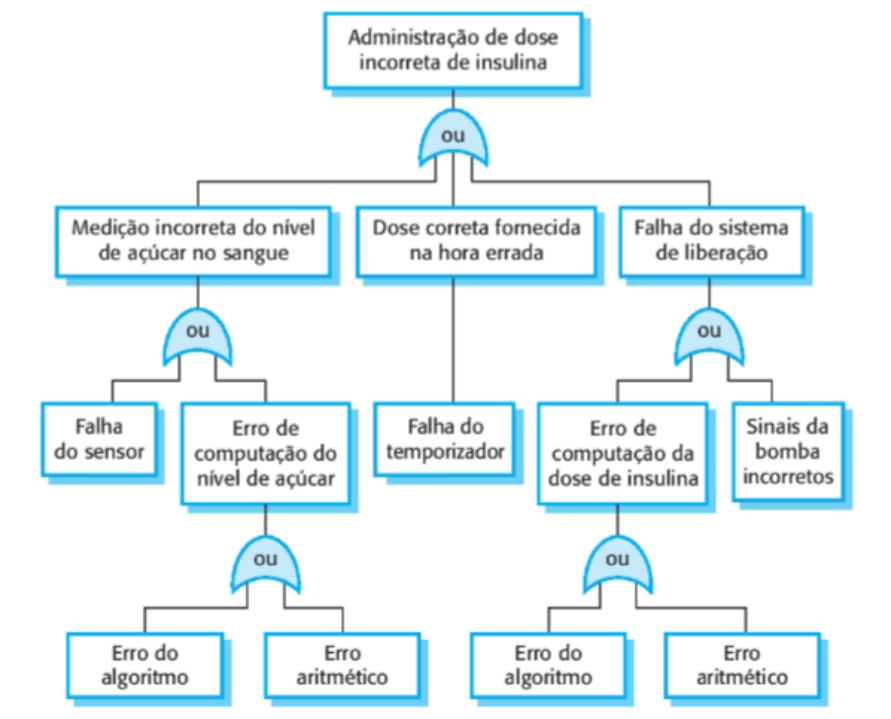
\includegraphics[width=0.55\textwidth]{arvore_de_Defeitos.png}
\end{frame}

% ===== SLIDE 45: ANÁLISE DOS RAMOS DA ÁRVORE =====
\begin{frame}{45) Análise dos Ramos da Árvore}
  \begin{itemize}
    \item \textbf{Ramo Esquerdo (Medição):} A falha pode vir do sensor físico ou de erros de computação (algoritmo ou ponto flutuante).
    \item \textbf{Ramo Central (Sincronismo):} Problemas de fornecer a dose cedo ou tarde demais resultam de falhas no temporizador.
    \item \textbf{Ramo Direito (Liberação):} Examina falhas no envio dos sinais corretos para a bomba ou erros no cálculo final da dose.
  \end{itemize}
  \vspace{0.4em}
  \begin{block}{Hardware vs. Software}
    Árvores de hardware podem sugerir requisitos de software para diagnóstico e correção (ex: autoverificação 4-6 vezes por hora).
  \end{block}
\end{frame}

% ===== SLIDE 46: 12.2.4 REDUÇÃO DO RISCO =====
\begin{frame}{46) 12.2.4 Redução do Risco}
  Três estratégias principais (geralmente combinadas):
  \vspace{0.5em}
  \begin{enumerate}
    \item \textbf{Proteção contra Perigos}: O sistema é projetado para que o perigo simplesmente não ocorra.
    \item \textbf{Detecção e Remoção}: Perigos são identificados e neutralizados antes do acidente.
    \item \textbf{Limitação de Danos}: Minimizar as consequências caso o acidente ocorra (ex: seguros, contenção física).
  \end{enumerate}
  \vspace{0.4em}
  \begin{alertblock}{Estado Seguro}
    Para a bomba de insulina, o \textbf{estado seguro} é o desligamento (injeção zero), pois no curto prazo isso não ameaça a saúde.
  \end{alertblock}
\end{frame}

% ===== SLIDE 47: TRATAMENTO DE ERROS E ESTADO SEGURO =====
\begin{frame}{47) Tratamento de Erros e Estado Seguro}
  Soluções para falhas de software na Bomba de Insulina:
  \vspace{0.5em}
  \begin{itemize}
    \item \textbf{Erro Aritmético:}
    \begin{itemize}
      \item Incluir tratamento de exceções para todos os erros possíveis.
      \item Ação padrão: \alert{desligar o sistema} e ativar alarme.
    \end{itemize}
    \item \textbf{Erro Algorítmico:}
    \begin{itemize}
      \item Comparar a dose calculada com a dose anterior (se for muito maior, pode ser erro).
      \item Monitorar a sequência de doses e limitar dosagens futuras excessivas.
    \end{itemize}
  \end{itemize}
\end{frame}

% ===== SLIDE 48: EXEMPLOS DE REQUISITOS DE SEGURANÇA =====
\begin{frame}{48) Exemplos de Requisitos de Segurança}
  \small
  \begin{itemize}
    \item \textbf{RS1:} O sistema não deve fornecer nenhuma dose única maior que a máxima especificada.
    \item \textbf{RS2:} O sistema não deve fornecer uma dose cumulativa diária maior que a máxima.
    \item \textbf{RS3:} O sistema deve incluir diagnóstico de hardware executado pelo menos 4 vezes/hora.
    \item \textbf{RS4:} O sistema deve incluir tratamento para todas as exceções identificadas.
    \item \textbf{RS5:} Um alarme audível deve soar em qualquer anomalia de HW ou SW.
    \item \textbf{RS6:} Em caso de alarme, o fornecimento de insulina deve ser suspenso até o reset manual.
  \end{itemize}
\end{frame}

% ===== SLIDE FINAL =====
\begin{frame}
  \centering
  \Huge Obrigado!\\
  \vspace{1cm}
  \large Dúvidas?
\end{frame}

% -------------
\end{document}
